\documentclass{sig-alternate-10pt}

\newcommand{\ttt}{\texttt}

\usepackage{graphicx}
\usepackage{changepage}
\usepackage{lipsum}
\usepackage{booktabs}

\title{FLASH\\Fast Linux Advanced Scheduler Hardware}
\author{
	Mark Aligbe \\
	    \email{ma2799@columbia.edu}
	\and
    Chae Jubb \\
        \email{ecj2122@columbia.edu}
}
\date{4 May 2015}

\begin{document}
\maketitle

\begin{abstract}
As accelerators become more common and necessary as a way to continue Moore's Law in the absence of Dennard Scaling, researchers explore segments of computation that can be improved with the aid of dedicated hardware. This paper presents FLASH, a hardware scheduler to take over the task of scheduling from the operating system. FLASH is able to make scheduling decisions in much fewer cycles as compared to modern operating system schedulers. The scheduling decisions it makes are just as good as those that would be made in software, but in much reduced time and without negatively impacting processor performance features. FLASH is designed to keep kernel modifications minimal, only requiring changes when the kernel scheduling interface changes.

\end{abstract}


\section{Introduction}
\label{sec:intro}
Traditional desktop operating systems are interactive, meaning that they serve as the primary interface between a user and a machine. Traditional server operating systems are batch-job oriented, meaning that processes are not pre-empted: a process continues until it exits or is forced to exit due to error. This preemption is one of the performance factors that contribute to greater process utilization on server operating systems as opposed to desktop operating systems. The reason why preemption is detrimental to CPU utilization is a combination of a few different reasons.

\paragraph{TLB and Cache}
The translation lookaside buffer (TLB) is a hardware structure that assists the memory management unit (MMU) of the CPU in translating virtual addresses into physical addresses. The TLB serves as a cache to look up commonly used virtual addresses and return the corresponding physical address. In computationally expensive portions of code, this unit is advantageous as it prevents unnecessary page lookups when the code is accessing a small region of memory. Likewise, the cache on a CPU provides good speedups to this kind of programs, as well as programs that have good data locality.

These structures work very well so long as the same process is in memory. When a context switch, changing from one process to another, is performed, the values of the cache and TLB are essentially invalidated. The new resident process must now wait for expensive memory accesses to bring in valid TLB entries and cache values. Before that process is even loaded, a scheduling algorithm must first decide which process to run next. This results in less than ideal processor utilization.

It is also difficult to make real time scheduling guarantees. In applications such as video playback, it is necessary that the playback process be scheduled consistently to ensure jitter-free playback. FLASH is able to make these guarantees due to its asynchronous computation and throughput. Additionally, FLASH minimizes the penalty to cache and TLB invalidation due to scheduler activity, while providing a complete scheduling interface.

\section{Scheduling in the Kernel}
\label{sec:sched_in_kernel}
% Mark
Modern desktop operating systems have to run hundreds of tasks, while providing a responsive interface to the user. This means that the CPU must be able to serve many interrupts a second, from various hardware devices, and service dozens or hundreds of background tasks while presenting a lagless experience to the end user. Each of these sources introduce potential sources of latency: interrupt handling \cite{regehr2007safe} requires many techniques in both hardware and software implementations to maintain relatively cheap and efficient scheduler design is an ongoing field of research \cite{wong2008cfs} \cite{park2008hardware} \cite{morton2004hardware}. We chose to focus on scheduling for our research as the potential benefits of scheduling in hardware in an operating system are not explored in the context of a desktop workload.

\subsection{History of Linux Schedulers}
The linux scheduler has gone through a few major design changes in its scheduler. Before the introduction of the $ O(n) $ scheduler in Linux 2.4, scheduler implementations simple and fast as CPUs themselves had not become as complex as compared to modern CPUs with simultaneous multi-threading (SMT) and symmetric multi-processing (SMP). These implementations were not scalable to multiple processors, so the $ O(n) $ scheduler was introduced to solve the problems introduced by SMP/SMT. The $ O(n) $ scheduler worked well so long as the number of tasks remained low, but as it had a single runqueue for all CPUs in a system, scaled poorly as the number of CPUs grew and as the number of processes grew (since it must iterate through the list of all processes to select a candidate).

The $ O(1) $ scheduler was introduced to solve the problem of large number of tasks. As the name implies, it is able to select a task to run in constant time. The $ O(1) $ scheduler achieves this efficiency by exploiting per-priority \textit{active} and \textit{expired} arrays for tasks. Tasks that are eligible to run are placed in the \textit{active} array and once a task has completed running it is placed in the \textit{expired} array. Thus, selecting a task is as fast as dequeuing the head of the highest priority array. Once the \textit{active} array is empty, the \textit{active} and \emph{expired} arrays are swapped by simply changing pointer directions. Unlike the $ O(n) $ processor, it had per-CPU runqueues, meaning task scheduling did not stall other CPUs. The $ O(1) $ was effective at its job, but was not a fair scheduler, was difficult to maintain through major kernel revisions, and its use of heuristics to determine the interactivity of a process was not without flaw. The CFS scheduler was introduced in Linux 2.6 as a replacement to solve the interactivity issues of the $ O(1) $ scheduler and introduce a simpler, but efficient scheduler.

\subsection{Implementation of CFS}
The CFS scheduler is conceptual simple; it aims to implement an ideal multi-tasking CPU \cite{cfsdesign}.
\subsection{Limitations}


\section{Related Works}
\label{sec:related_works}
Previous hardware scheduling units focus completely on embedded systems with
a fixed number of tasks each with fixed priority
\cite{kuacharoen2003configurable, morton2004hardware, nacul2007hardware, nakano1995hardware,
park2008hardware}.  Scheduling under these fairly restrictive constraints is
greatly simplified with respect to desktop scheduling as there is a much
more defined ordering between tasks.

Additionally, there is often a small number of tasks relative to a desktop
environment.  This means that much simpler algorithms may be used in an
attempt to approximate the optimal task ordering.

The major novel challenge in escalating to a desktop Linux is handling the
dynamic, unbounded (from a realistic hardware perspective) number of tasks.
The initial FLASH prototype addresses this in an unsatisfying way: by
arbitrarily fixing the number of tasks that can be managed with its
scheduling policy.  As discussed in detail in Section~\ref{sec:future},
future iterations will remove this restriction by reserving a small section
of memory.

Because we aim to support an unbounded number of tasks, we must implement
a scheduler comparable to the default CFS currently used by the kernel.
While a simpler implementation than the kernel default, the FLASH scheduler
is implemented in accordance with the major principle of CFS
\cite{wong2008cfs}.

We should also consider the architecture of previous hardware schedulers.
Many of the previously cited works were designed either as ASICs
(Application Specific Integrated Circuits) or on FPGAs (Field Programmable
Gate Arrays) rather than a general purpose CPUs.  This makes scheduling of
resource usage slightly different in that there is not always an overhead of
a context switch: we may simply be deciding which process can use
a particular multiplier.


\section{FLASH Architecture}
\label{sec:arch}
% Chae
The FLASH hardware unit is built with ease of replacement of the usual
software implementation in mind.  The major addition we add over a standard
scheduler is the ability for the external scheduler itself to raise an
interrupt to indicate a tick. Either at this tick or when a process is
requested, FLASH will provide the process ID of the task to the run next.
Figure~\ref{fig:arch_overview} gives an overview of the system architecture.

\begin{figure}
	\begin{center}
		%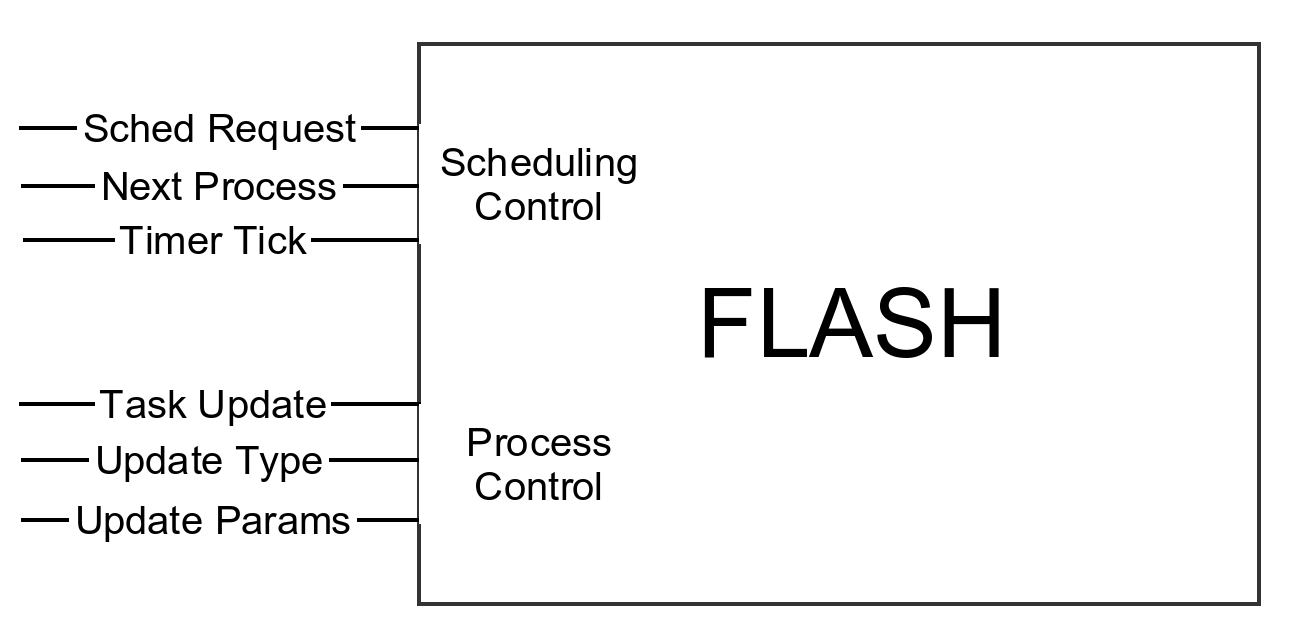
\includegraphics[width=0.65\textwidth]{fig/flash-diagram.png}
		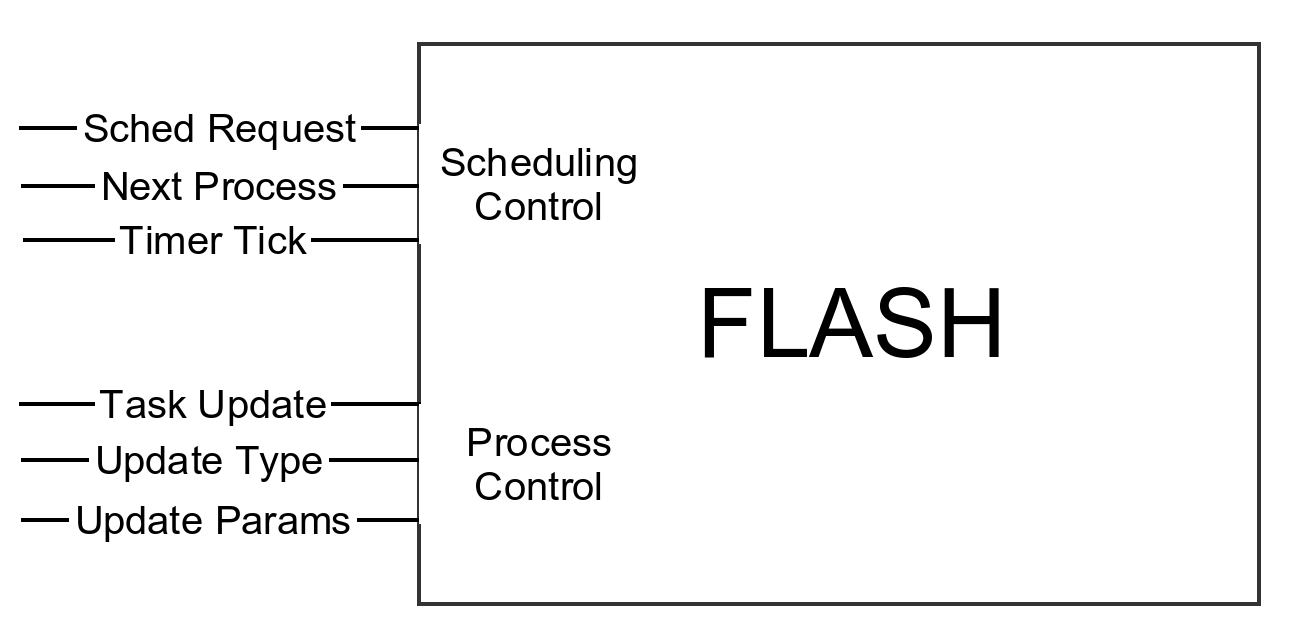
\includegraphics[width=0.9\linewidth]{fig/flash-diagram.png}
		\caption{
			FLASH System Architecture: Interface.  Note the distinction between
			the \emph{Process Control} and \emph{Scheduling Control} Interfaces.
		}
		\label{fig:arch_overview}
	\end{center}
\end{figure}

\subsection{Improvements}
FLASH provides improvements over the CFS software solutions.  The most
notable potential advantage is in speed.  Having a separate hardware unit
allows the CPU to be running tasks at the same time the choice of next task
is being prepared.  This way it can be immediately read without having to
wait for a computation.

Additionally, data structures are maintained on a separate data path.  This
means that scheduling computations will not pollute the usual cache
hierarchy or TLB.  As cache misses are costly, eliminating a small class of
them will directly correlate to a performance increase.  This will be
especially true as modern processor hardware (newer versions of x86 and ARM)
have more effective TLBs that are not, for example, completely flushed on
a context switch\cite{neiger2006intel}.  FLASH allows program data a larger
share of the cache hierarchy and TLB.

Increasingly, desktop machines are being used as virtualization platforms.
The problem of TLB hit rate is especially relevant with the added number of
virtual memory spaces so it is important that the TLB stay as intact as
possible through context switches.

\subsection{Scheduling Algorithm}
As previously mentioned, in order to best schedule the set of eligible
tasks, we use the same fundamental algorithm to which the Linux kernel
defaults: the Completely Fair Scheduler.  The kernel's implementation
fundamentally relies upon red-black trees.

However, implementing a red-black tree in hardware with a fixed amount of
memory would be prohibitively expensive.  For this reason, the FLASH
implementation utilizes a simple unordered array.  Because there are
typically very few tasks, the cost of keeping and constantly reorganizing an
ordered data structure would would outweigh a simple iteration.  Further, we
must importantly note that this lookup in hardware will be much quicker than
in software, given that the data is stored in a single monolithic,
low-latency memory.  Even more convincing is the ease with with
parallelization of lookup can be implemented using hardware.

FLASH does, however, retain the core functionality of the CFS basis
algorithm.  Scheduling decisions are made using the notion of virtual
runtime.   Just as in the Linux implementation, virtual runtime is
calculated as a weighted physical runtime based upon the priority of the
task.  FLASH uses the same relative weighting as Linux.

We now describe in more detail both the interface and internal
implementation of the scheduling unit.

\subsection{FLASH Interface}
At its most basic, the hardware interface is given by two major segments:
\emph{scheduling control} and \emph{process control}.  Together these two
segments allow processes to be scheduled based on an up-to-date accounting
of process status, kept via the process control interface.  The scheduling
controller interface sends timer tick interrupts and serves incoming
requests for new processes to run.

\subsubsection{Process Control Interface}
Let us first focus deeply on this process control interface.  It is here
that FLASH is given information to hold the proper state of all running
processes.  Currently, we store process id (PID), priority, and state
triples as passed through the interface using a standard four-phase
handshake.

\paragraph{Consistency} A major hurdle with offloading scheduling decisions
to a dedicated piece of hardware is ensuring consistency between the data
structures maintained by the software kernel (again, here Linux) and the
hardware unit.

We cannot completely offload the data about processes to hardware most
obviously because of sheer size of objects like the \ttt{task\_struct} as
well as their high use by modules other than the scheduler.  We must,
though, retain some structure in FLASH memory so that it may make even the
most basic scheduling decisions.

For this reason, we expect each update in process priority or state to be
communicated to FLASH so it may continue making accurate scheduling
decisions.

\subsubsection{Scheduling Control Interface}
In addition to the process control interface, FLASH provides a scheduling
control interface, responsible for providing the software with tasks to be
run.  We can further subdivide this interface into two subparts: scheduling
requests and timer ticks.  Making replacement of software more
straightforward, these subparts directly correspond to the two main modes of
tasks switching in the Linux Kernel.

\paragraph{Scheduling Requests}
Often a running process will want to do something (such as disk I/O) that
requires yielding the processor.  When this occurs, the Linux kernel will
call \texttt{schedule()}.  We modify this schedule function to interact with
our scheduling control interface, more specifically the portion dealing with
scheduling requests.

A scheduling request will be received using a standard four-phase handshake.
At this point, using methods explained in Section~\ref{sec:FLASH_impl}, the
next task to be run is selected and returned to the software.

\paragraph{Timer Tick}
FLASH also provides functionality to raise an interrupt via a timer tick.
For simplicity and fully encapsulating scheduling logic, we export the
generation of the timer tick to this hardware unit.  At a specified time
interval, FLASH will raise a timer interrupt and provide the software with
the next task to be run.

\subsection{FLASH Implementation}
\label{sec:FLASH_impl}
FLASH aims to implement a CFS scheduling algorithm\footnote{The current
implementation is a prioritized round robin algorithm.}, allowing
transparent replacement of the current software implementation.  Internally,
we have two front-end modules, each corresponding to a segment of the
interface (process control and scheduling control). Those front-end modules
connect to back-end modules which regulate and control access to the backing
internal data structures.  We see this internal implementation architecture
described in Figure~\ref{fig:impl_overview}.

\begin{figure*}
	\begin{center}
		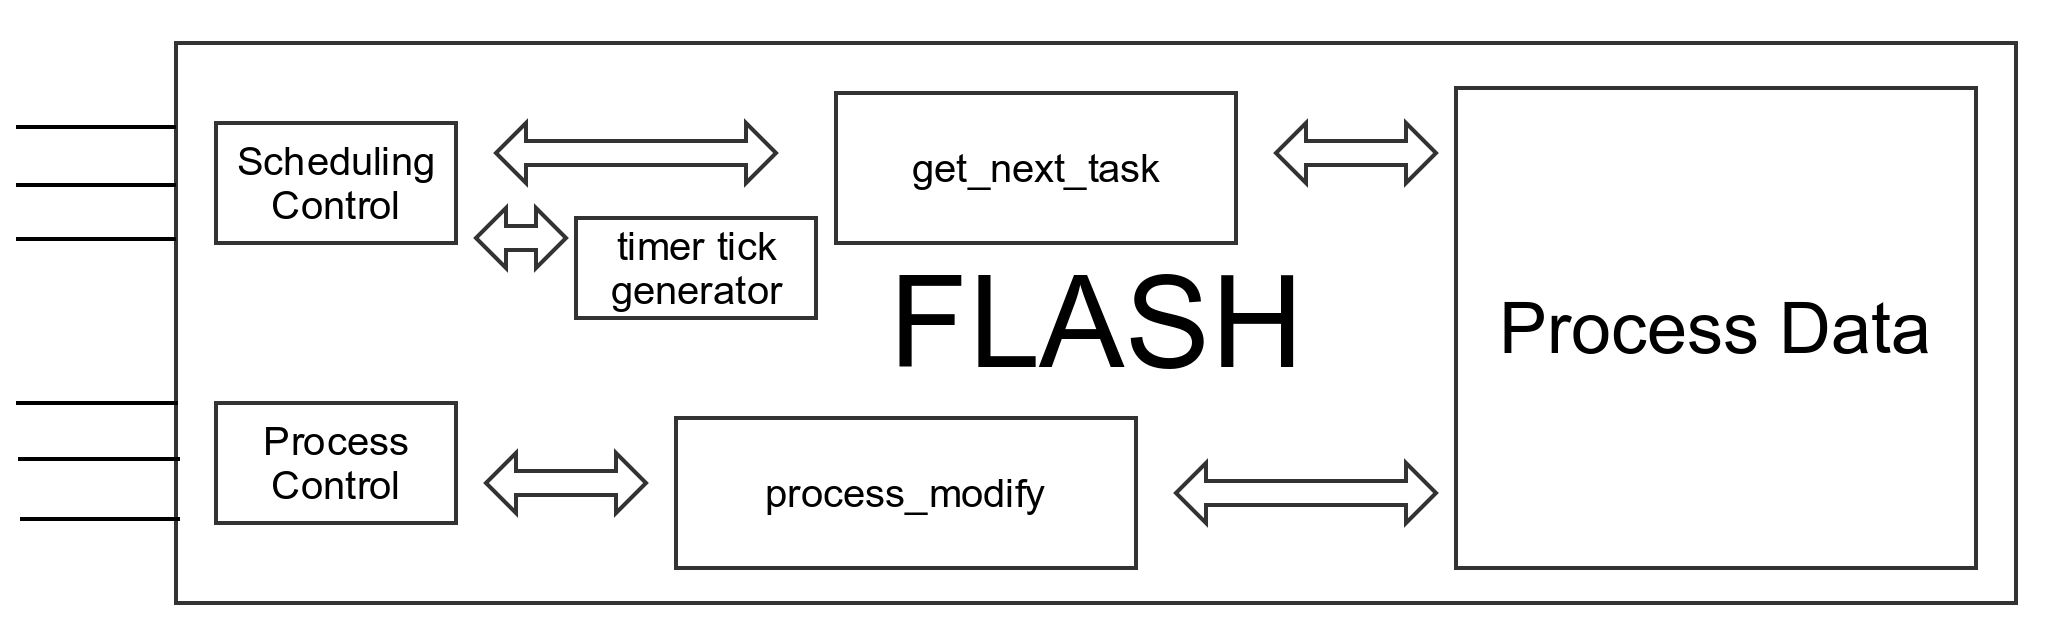
\includegraphics[width=0.9\textwidth]{fig/flash-impl.png}
		%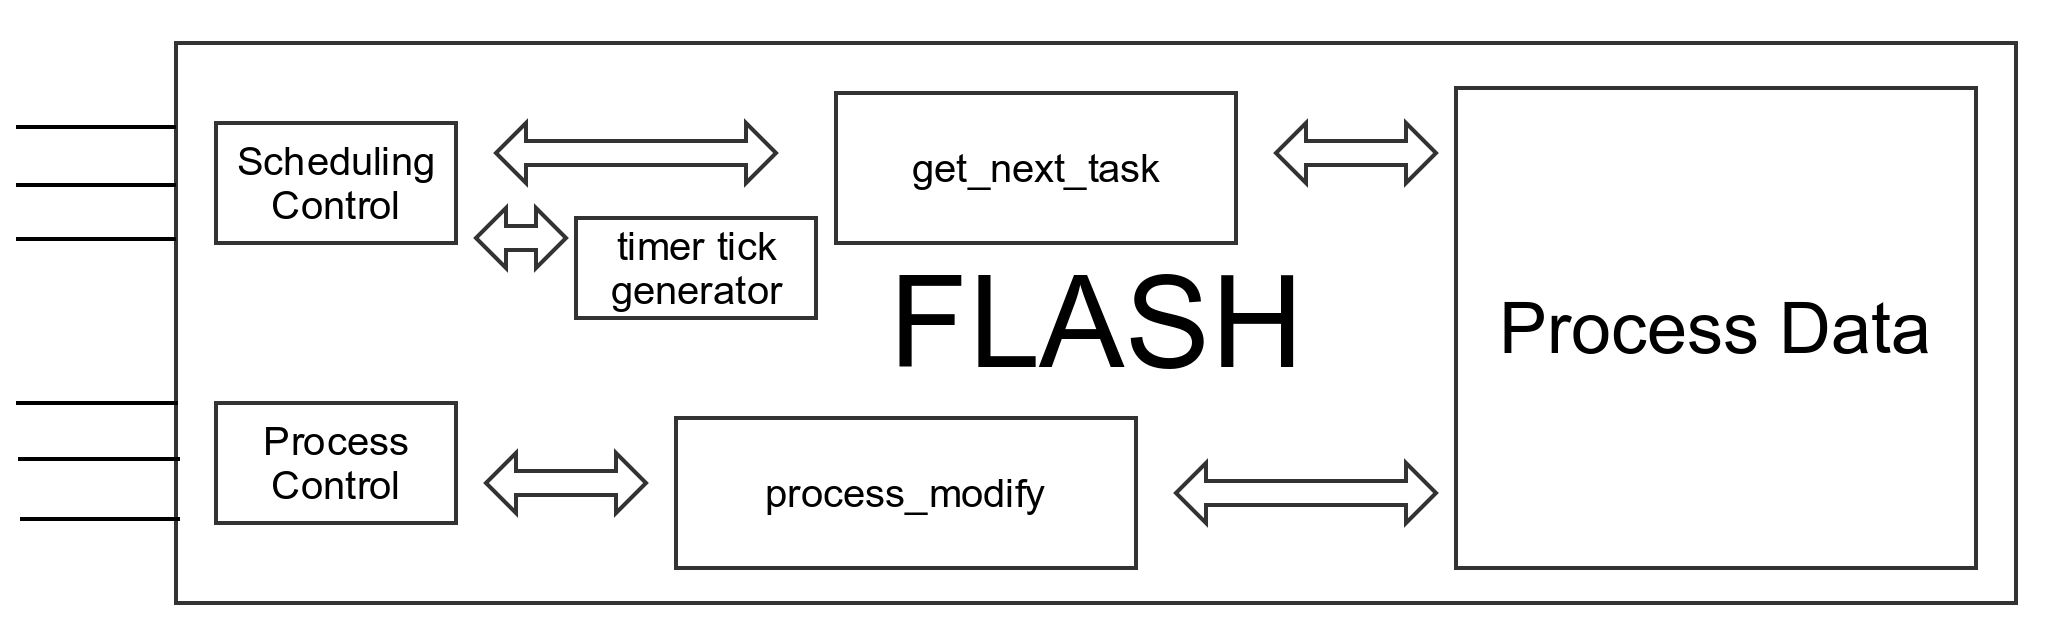
\includegraphics[width=0.9\linewidth]{fig/flash-impl.png}
		\caption{
			FLASH System Architecture: Implementation.  Notice the division
			between the front-end, back-end, and process data modules.  This
			allows tightly regulated access to backing process data store.
		}
		\label{fig:impl_overview}
	\end{center}
\end{figure*}

\subsubsection{Front-End Modules}
As mentioned above, we have a front-end module for each segment of the
interface.  Each of these modules is quite simple.  The module corresponding
to the scheduling control interface has two jobs: responding to scheduling requests
as well as passing on timer ticks generated by a different internal module.
Both of these require querying for the next task to be run.

The second front-end module corresponds to the process control interface.
It will simply communicate through the incoming request and update the
backing store of process state.

\subsubsection{Back-End Modules}
The FLASH back-end modules serve to regulate access to the backing data
store.  This is done via two modules: a reading module and a writing module.
The process control datapath is connected through the writing module as this
interface is used to modify the state of processes.

Additionally, we have a simple reading module connected to the scheduling
control interface.  This regulates reads to the backing data store in order
to determine the next process that ought to be run.

\subsubsection{Storing Process State}
The current FLASH implementation is a basic version of CFS.  We do not use
the same type of implementation as the Linux kernel because implementing
red-black trees in hardware would be prohibitively complex.  Instead we use
a series of simple queues that are sorted with priority in mind.

The FLASH scheduling algorithm, like CFS, will keep record of the runtime of
the process as well as a \emph{virtual runtime}.  This virtual runtime is a
weighted accounting of the actual runtime based on priority of the process.
Scheduling decisions are made based on the virtual runtime, as in CFS.

\paragraph{On Red-Black trees}
While using a red-black tree would allow the implementation to be
algorithmically faster, actual runtime in software will likely be higher
than iterating through a simple queue implemented in hardware.  Firstly,
hardware will simply be faster than software as it is more easily
parallelizable.  The hardware can parallelize comparisons in logarithmic
time, whereas an iteration in software will take linear time.

Secondly, traversing the red-black tree in software will not have ideal cache
performance. Switching to a self-contained hardware module will not have any
cache considerations because that hardware unit will have a single
monolithic memory.

\paragraph{What do we store?}
In addition to storing the PID, priority, and state, we also have a few
fields used to store internal state necessary to keep the CFS implementation
completely fair.  These fields most importantly include a notion of virtual
runtime.  Other fields are for bookkeeping reasons.

\subsection{Summary}
Together the interface and implementation of FLASH provide an easily
integrable scheduling module.  The kernel will interface with the hardware
unit in the same way that the software scheduler does.  Additionally, FLASH
implements the fundamental algorithm of the current default Linux scheduler
CFS, relying upon the notion of a priority-weighted virtual runtime.


\section{Integration}
\label{sec:integration}
% intro stuff here
\subsection{Cyclone V}
% Mark
\begin{figure}
	\begin{center}
		%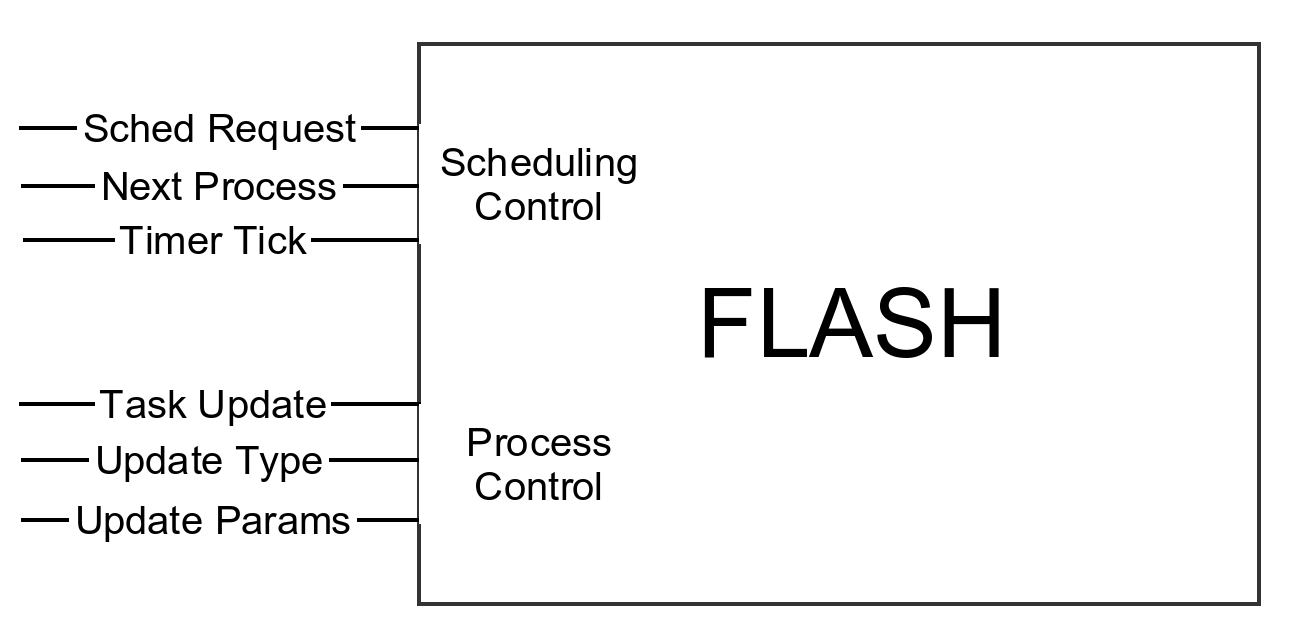
\includegraphics[width=0.65\textwidth]{fig/flash-diagram.png}
		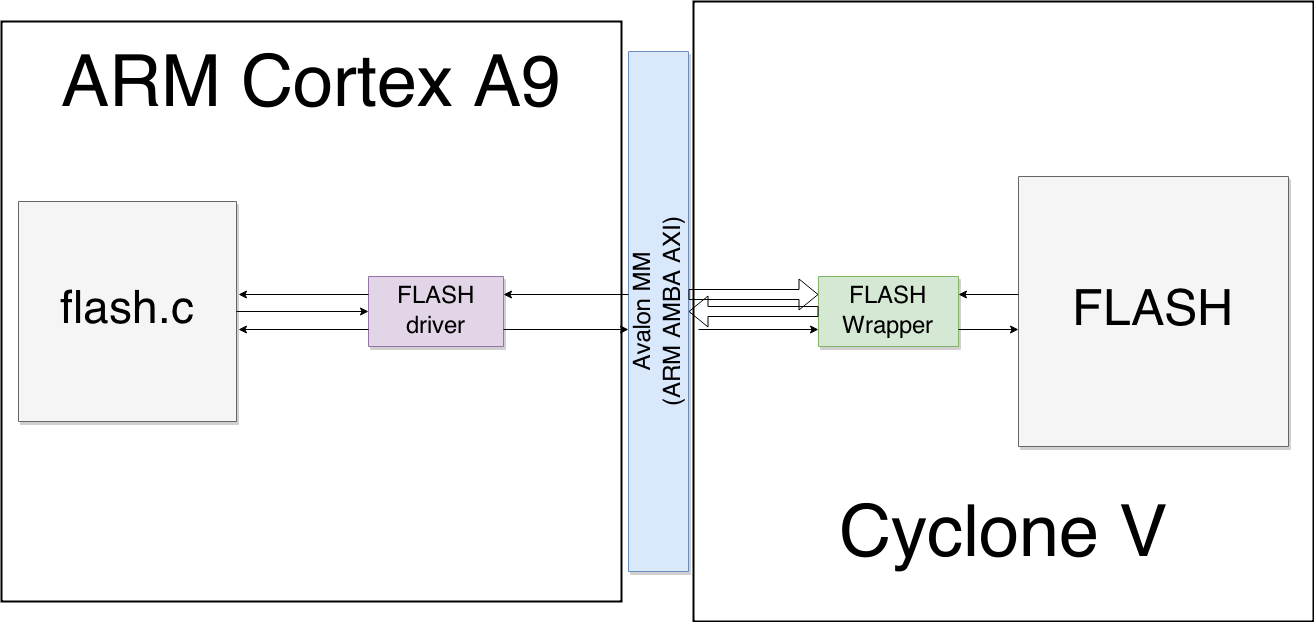
\includegraphics[width=0.9\linewidth]{fig/sockit-architecture.png}
		\caption{
			Arrow SoCKiT high level overview. The embedded ARM processor is connected to the FPGA fabric via a ARM's AMBA AXI interface, on top of which runs Altera's Avalon MM interface.
		}
		\label{fig:sockit_overview}
	\end{center}
\end{figure}


\subsection{Kernel mods}
% Chae
\lipsum[1-3]


\section{Applications}
\label{sec:apps}
% Mark
\lipsum[1-3]


\section{Engineering Experiences}
\label{sec:eng_exp}
% both
\lipsum[1-3]

\section{Future Work}
\label{sec:future}
\subsection{DMA}
\subsection{No HZ Interrupt}

\section{Conclusion}
\label{sec:conclusion}
\lipsum[1]

\nocite{*}
{
	\bibliographystyle{abbrv}
	\bibliography{ref}
}

\end{document}
